\entry{2026-10-09}{Derivative-aware bank (C3, complete): the bank is not the bottleneck}

Lane \texttt{2026-10-08-jcp-smooth-bank}, last commit \texttt{12f620782}, mirror \texttt{8ede69cba}. Jobs 5016275 and 5027733 (training, 4$\times$ A100 each); 5027022 and 5037650 (evaluation). All steps were Codex-gated. The report audit confirmed all fixes except four minor presentation items. Report: \path{worktrees/2026-10-08-jcp-smooth-bank/experiments/jcp-smooth-bank/report.md}. \textbf{Provisional:} first-order references, one training seed per recipe, development and validation cohorts only.

\subsection*{Findings}
\begin{itemize}
\item \textbf{Smoother banks need no fewer points at the acceptance bars.} In the accurate setting every bank needs Gauss $56^2$. The point count there is set by the $M=1536$ high-frequency tests, not by the bank: with only the first 320 tests, Gauss $32^2$ is already near the bar.
\item \textbf{Smoothness pays only in the high-accuracy tail.} At $256^2$ points the worst $\rho$ is $3.2\times10^{-6}$ for $\sigma=1$, against $3.1\times10^{-4}$ for the baseline, with no loss of representation accuracy.
\item \textbf{Sobolev training improves the bank's derivatives but not the ROM.} The median gradient error falls by 53, 70 and 74\,\% for $\lambda = 0.01, 0.1, 1$. The ROM error against the space-only reference does not improve (it rises by 62\,\% at $\lambda=1$).
\item \textbf{All banks sit at the time-stepping floor} against the space+time reference: 2.74--2.97\,\% in the accurate setting.
\item \textbf{Coarse-data control.} A bank trained only on 129-node data gives 0.83\,\% worst error against the space-only reference, against 7.58\,\% for the 129-node FOM and 4.12\,\% for the 257-node FOM, in the accurate setting. So finer training data were not necessary for the gain. This holds in the accurate setting only, and the cause is not isolated. The same bank needs 16384 points.
\end{itemize}
\begin{center}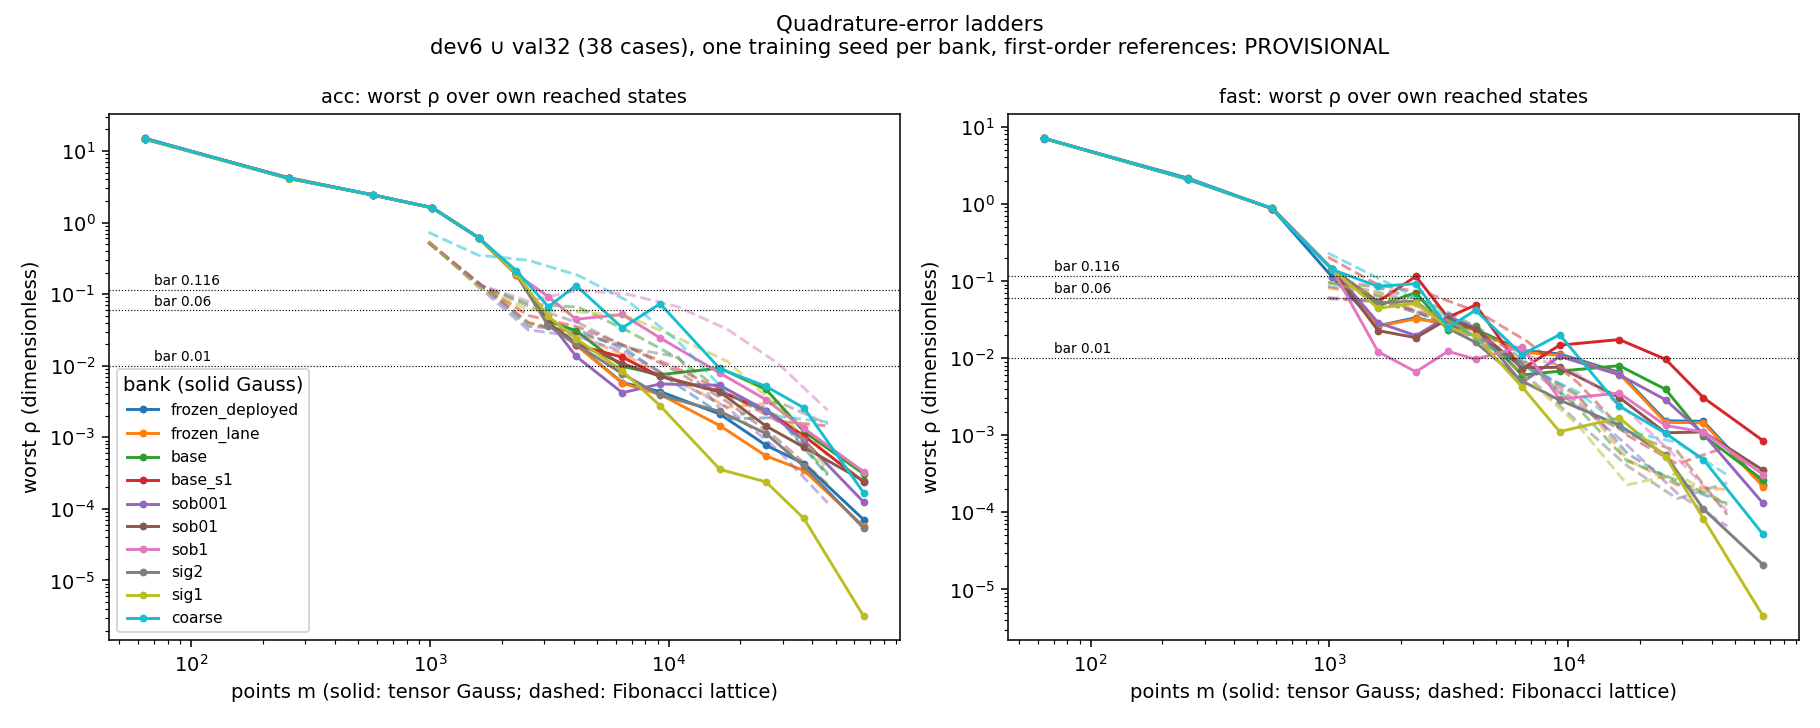
\includegraphics[width=0.8\linewidth]{figs/c3_ladders.png}\end{center}

\subsection*{Corrections}
\retracted{runs/SUMMARY-R3.md describes the wrong training job; the deployed bank is r3a. The 2D lane's training-overlap check used the wrong draw (the cohorts were re-verified as disjoint). Retrains are not bitwise reproducible without deterministic XLA flags. In the fast setting, the 2D numbers depend on the column-ordering procedure (3.45\,\% vs 4.51\,\%).}

\subsection*{Week summary (8--9 October)}
\begin{itemize}
\item \textbf{Mechanism (A):} the accuracy comes from the exact gradient; classical quadrature makes it cheap.
\item \textbf{Second-order time stepping (C2):} the clear win. The median error falls about 9$\times$ at equal cost, and the matched speed-up against a fair second-order FOM rises from 1.8$\times$ to 3.7$\times$.
\item \textbf{Wider bank (C1)} and \textbf{smoother or Sobolev bank (C3):} each represents the solution better, but the ROM error does not follow. The bank is no longer the bottleneck.
\item \textbf{Next:} second-order stepping with the wide bank, measured against second-order references (the E0 lane); a fixed-sweep second-order 3D solver; a test space with lower mixed frequencies.
\end{itemize}
